
\begin{minipage}[t]{9.5cm}
\center
	\textbf{DZRD}: $\boxed{x_{k+1}=A_d\cdot x_k + B_d\cdot u_k \qquad y_k=C x_k (+ D\cdot u_k)}$\\
	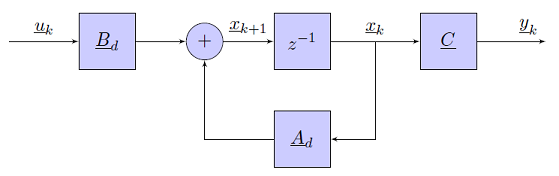
\includegraphics[width=9cm]{Content/Divers/diskretblockschaltbild.png}\\

\end{minipage}
\begin{minipage}[t]{9.5cm}
\center
	\textbf{Zyklisch Falten}
	\begin{enumerate}
		\item Beide Vektoren mittels Zero-Padding auf Zielvektorl�nge bringen $(N+M-1)$
		\item Ein Vektor spiegeln und zyklisch verschieben (Werte die �berlappen wieder hinten anh�ngen)
	\end{enumerate}
\end{minipage}

%\vspace{-0.5cm}

\begin{minipage}{3cm}

\vspace{-0.2cm}

	\textbf{Mason}\\
	$\boxed{T_{ij} = \frac{\sum\limits_k P_k\cdot\Delta_k}{\Delta}}\quad$
\end{minipage}
\begin{minipage}{15.5cm}

	\vspace{0.2cm}
	$P_k$ Vorw�rtspfad k\\
	$\Delta$ = 1- (Summe aller Schleifen) + ($\sum{}$ aller Produkte zweier
	Schleifen, die sich nicht ber�hren) -$\ldots$
	$\Delta_k$ = 1- (Summe aller Schleifen die $P_k$ nicht ber�hren) +$\ldots$ 
\end{minipage}\\
$h(n)$ berechnen: $\frac{Z(z)}{N(z)}= h[0]+h[1]z^-1+h[2]z^-2+h[3]z^-3+...$